
\documentclass[a4paper,12pt]{article}

\usepackage[a4paper, total={6in, 8in}, left=30mm]{geometry}
\usepackage{pdfpages}

\usepackage{cmap}
\usepackage[T2A]{fontenc}
\usepackage[utf8]{inputenc}
\usepackage[english,russian]{babel}
\usepackage{fancyhdr}
\usepackage{minted}
\usepackage{hyperref}
\usepackage{amsmath}
\usepackage{graphicx}

\hypersetup{
  pdfborderstyle={/S/U/W 1}
}

\graphicspath{{./images/}}

\pagestyle{fancy}
\fancyhf{}
\lhead{Антон Завьялов, ПИ-72}
\rhead{\textbf{Лабораторная №13}}
\cfoot{\thepage}

\makeatletter
\def\@seccntformat#1{%
  \expandafter\ifx\csname c@#1\endcsname\c@section\else
  \csname the#1\endcsname\quad
  \fi}
\makeatother

\begin{document} % Конец преамбулы, начало текста.
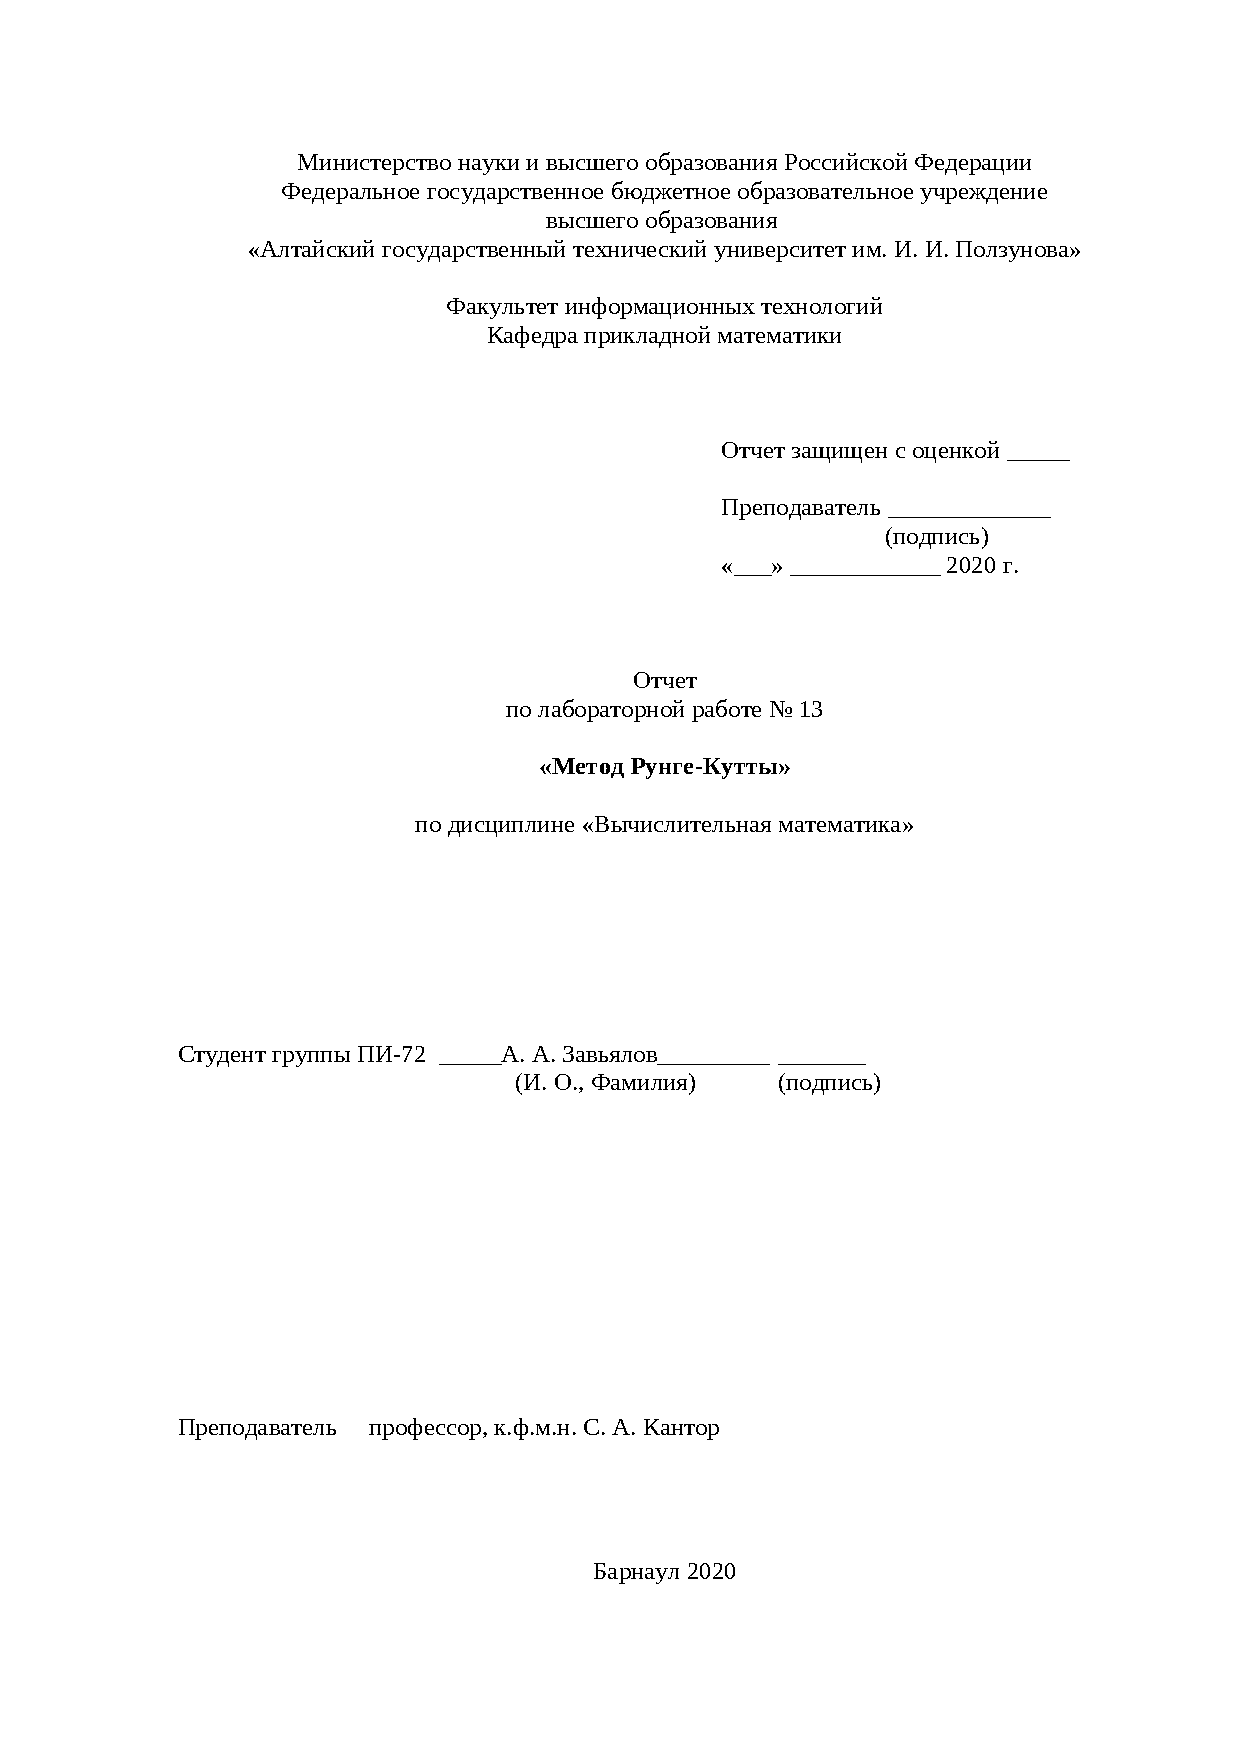
\includepdf[pages={1}]{title.pdf}

\section{\normalsize{Задание к лабораторной работе}}
\begin{flushleft}
    \begin{itemize}
        \item Составить программу решения задачи Коши для \textbf{системы} \textit{n} обыкновенных дифференциальных уравнений методом Рунге-Кутта четвертого порядка точности. В программе предусмотреть два режима работы - с постоянным шагом и автоматическим выбором шага. В основу автоматического выбора шага для студентов, чей номер зачетной книжки четный, положить метод Рунге, а для тех, у кого номер нечетный, - вложенный метод.\linebreak[2]Правые части системы уравнений задать в программе, а остальные параметры: начальные данные, промежуток интегрирования, шаг, точность \(\epsilon\) - в файле или диалоге в процессе выполнения программы.
        \item Вывести в файл таблицу значений функций, получить графики решений.
        \item Для тестовых примеров, решение которых известно, наряду с графиками приближенного значения y построить графики точного решения \textbf{u} и получить в сопоставимых с приближенным решением точках \(x_j\) таблицу значений функции. Вычислить норму глобальной погрешности \(\displaystyle\max_{i=1,...,n}\max_j\mathopen|y_i(x_j)-u_i(x_j)\mathclose|\).
        \item Путем проведения численных экспериментов исследовать зависимость нормы глобальной погрешности от величины шага (для вычислений с постоянным шагом) и точности \(\epsilon\) (для вычислений с переменным шагом).
        \item Найти, используя Вашу программу с постоянным шагом, решение задачи\linebreak\[u^{'} + 30u = 0, u(0) = 1, 0 \le x \le 1.\]\linebreak Расчеты провести дважды, первый раз разбить промежуток интегрирования на 10 частей, а второй на 11. Объяснить, почему результаты расчетов качественно отличаются.
    \end{itemize}
\end{flushleft}
\begin{flushleft}
    \textit{Указание} Для тестирования программы можно рассмотреть следующую задачу Коши\linebreak \[u^{'}=f^{'}(x)+p(u-f(x)), 0 \le x \le l, u(0) = f(0).\]\linebreak Здесь \(p \ne 0\) - заданная константа, а \(f(x)\) - заданная гладкая функция. Очевидно, что решением этой задачи Коши на отрезке \([0,l]\) является функция \(u=f(x)\). Рекомендуется исследовать поведение численного решения в зависимости от величины и знака коэффициента \(p\).
\end{flushleft}

\section{\normalsize{Краткое описание метода, расчётные формулы}}
\begin{flushleft}
    Имеется задача Коши для системы обыкновенных дифференциальных уравнений:
    \[u'(x) = f(x, u),\]\[u = (u_1, ..., u_n), f = (f_1, ..., f_n),\]\[u(x_0) = u_0.\]
    Необходимо найти решение системы с заданным начальным условием на некотором отрезке.
    \linebreak\linebreak
    Метод Рунге-Кутты 4 порядка точности позволяет построить таблицу значений $u$ по следующим формулам:
    \[y_{n+1} = y_n + \frac{1}{6}(k_1 + 2 k_2 + 2 k_3 + k_4),\]
    \[k_1 = hf(x_n, y_n),\]
    \[k_2 = hf(x_n + h/2, y_n + k_1/2),\]
    \[k_3 = hf(x_n + h/2, y_n + k_2/2),\]
    \[k_4 = hf(x_n + h,y_n + k_3).\]
    \linebreak
    \textit{Автоматический выбор шага проводится по следующей схеме:}
    \begin{enumerate}
      \item Вычисляется \(err = \mathopen|\frac{\psi}{M}\mathclose|,\) в данной работе \(\psi = E = \frac{2}{3}(k_1 - k_2 - k_3 + k_4)\) - контрольный член Егорова, \(M = 1\) - масштабирующий множитель (\(M = 1\) для вычисления абсолютной погрешности).
      \item Вычисляется \(h_{new} = h * min(facmax, max(facmin, fac(\frac{\epsilon}{err})^{1/(s+1)}))\), \(1.5 \le facmax \le 5\), \(0.2 \le facmin \le 0.7\), \(fac \in \{0.8, 0.9\}\), \(s = 4\).
      \item Если на шаге \(err \le \epsilon\), решение считается принятым, расчеты продолжаются с новым шагом $h_{new}$, иначе результаты на шаге отбрасываются, вычисления повторяются с новым шагом $h_{new}$, для этой итерации полагается $facmax = 1$.
    \end{enumerate}
\end{flushleft}


\section{\normalsize{Текст программы с комментариями}}
Кроме расположенных ниже листингов, исходный код можно посмотреть по адресу: \url{https://github.com/andiogenes/differential-equations/tree/master/runge-kutta-method}
\linebreak\linebreak\textbf{Entry.scala}
\inputminted[breaklines]{scala}{../src/main/scala/Entry.scala}

\textbf{RungeKuttaMethod.scala}
\inputminted[breaklines]{scala}{../src/main/scala/RungeKuttaMethod.scala}

\textbf{CliParser.scala}
\inputminted[breaklines]{scala}{../src/main/scala/CliParser.scala}

\section{\normalsize{Тестовые примеры}}
\begin{flushleft}
  \begin{enumerate}
    \item 
      \(u^{'} + 30u = 0, u(0) = 1, 0 \le x \le 1\)\linebreak\linebreak
      \textit{Сетка из 10 точек:}\linebreak
      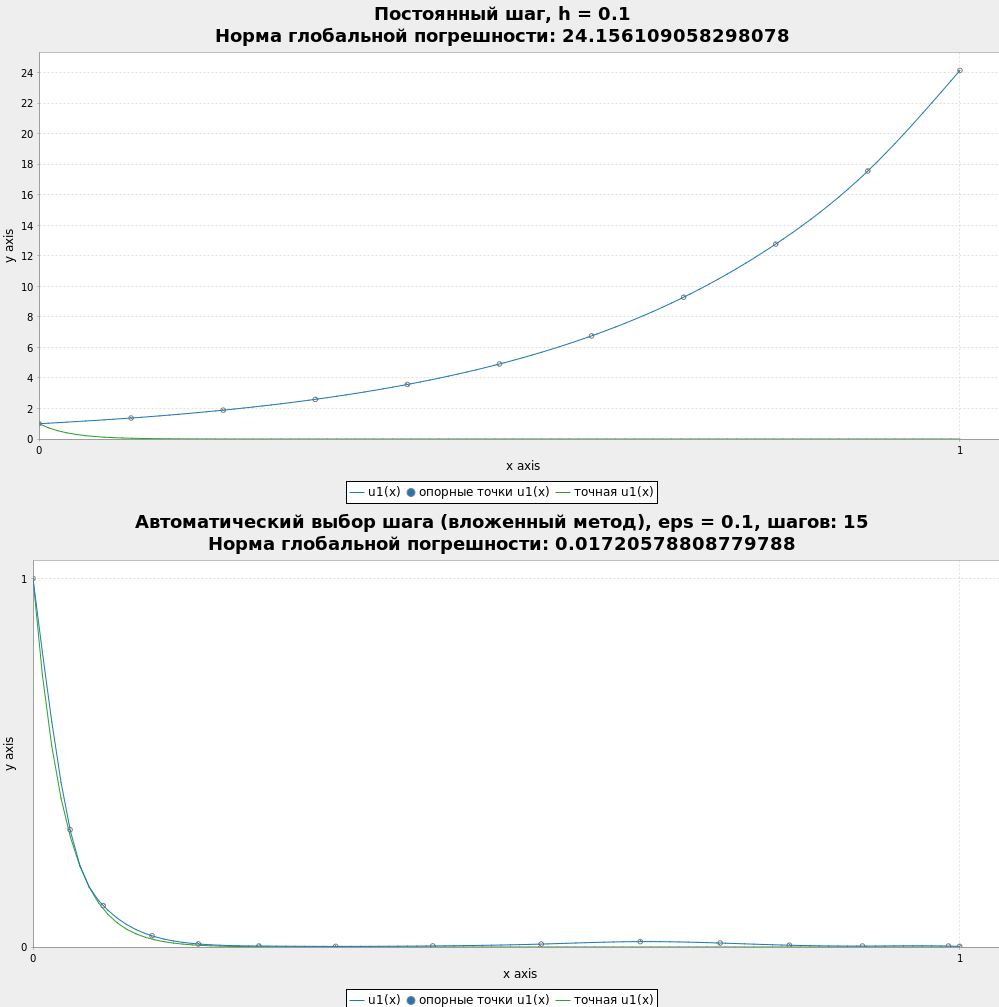
\includegraphics[scale=0.325]{10_segments.png}\linebreak
      \textit{Сетка из 11 точек:}\linebreak\linebreak
      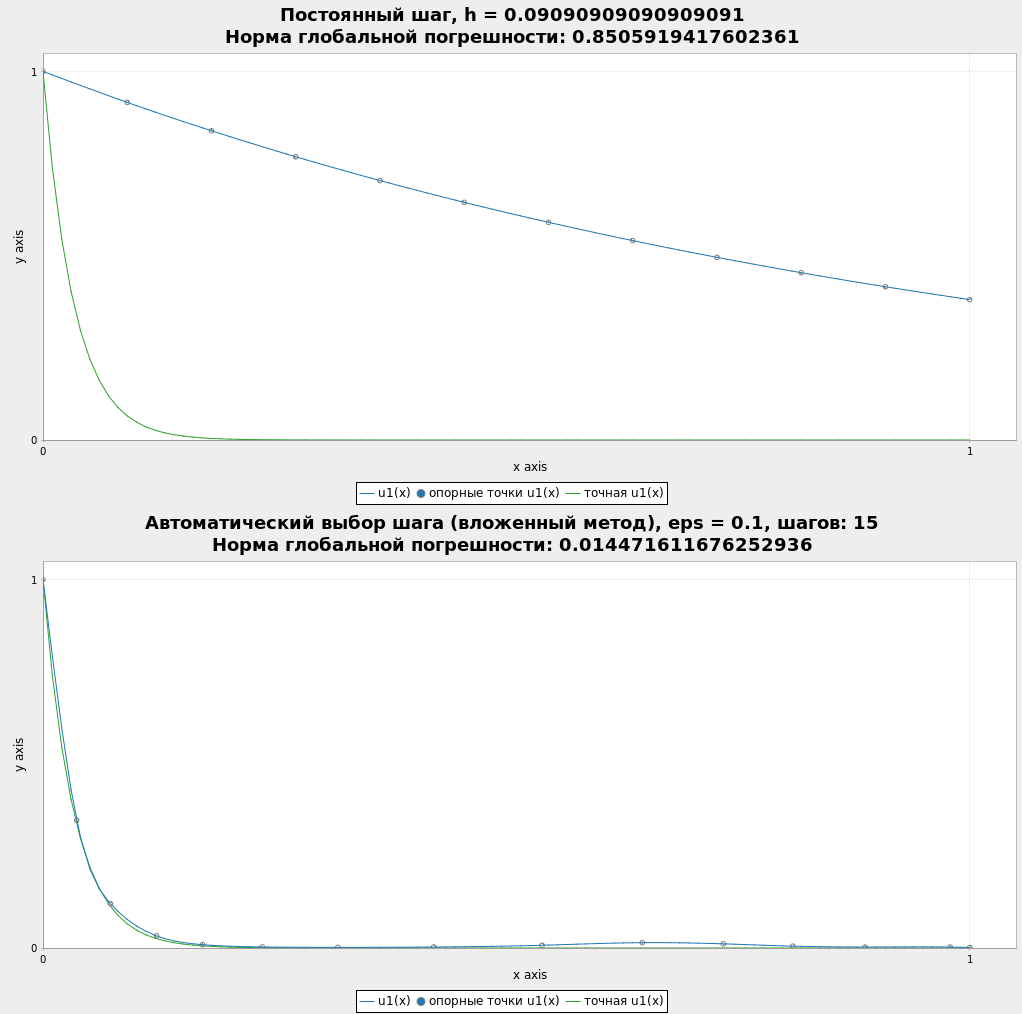
\includegraphics[scale=0.325]{11_segments.png}\linebreak
      \textit{Таблица значений для сетки из 10 точек:}\linebreak\linebreak
      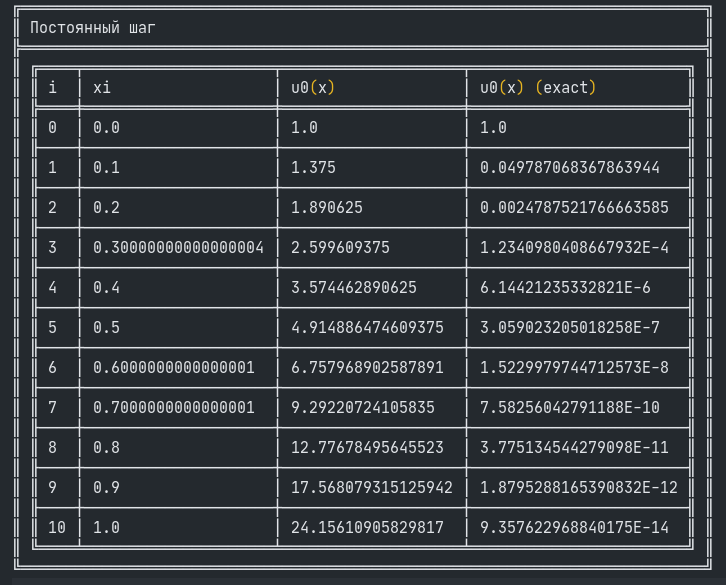
\includegraphics[scale=0.325]{10steps.png}\linebreak
      \textit{Таблица значений для сетки из 11 точек:}\linebreak\linebreak
      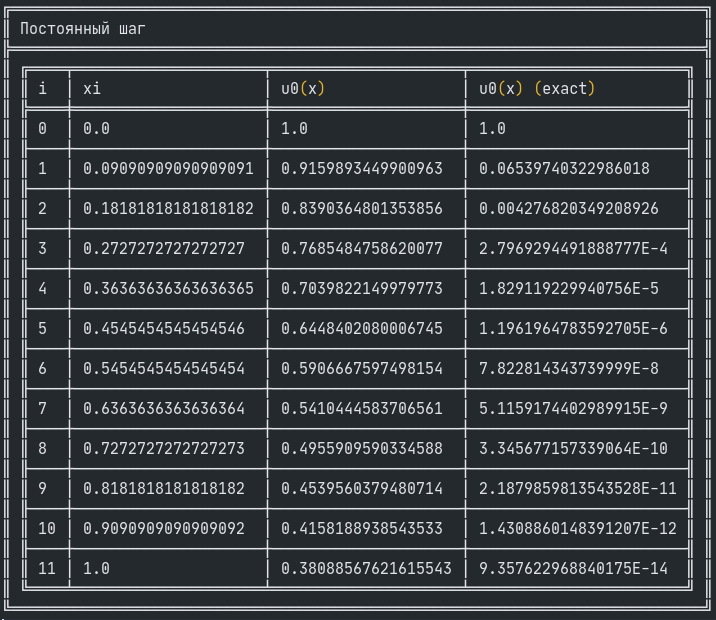
\includegraphics[scale=0.325]{11steps.png}\linebreak\linebreak
      Если взять $h = 0.1$, $f = -30u$, то \(u_{n+1} = u_n + \frac{3}{8}u_n\), и очевидно, что \(\lim_{n\to\infty} u_n = \infty\).\linebreak\linebreak
      При $h = \frac{1}{11}$: \(\frac{1}{6}(k_1 + 2k_2 + 2k_3 + k_4) < 0\) и $u_n$ убывает на \([0, 1]\).
    \item
      \textit{Исследование зависимости нормы глобальной погрешности от шага и точности (используется задача из прошлого пункта)}\linebreak\linebreak
      $h = 0.05:$\linebreak\linebreak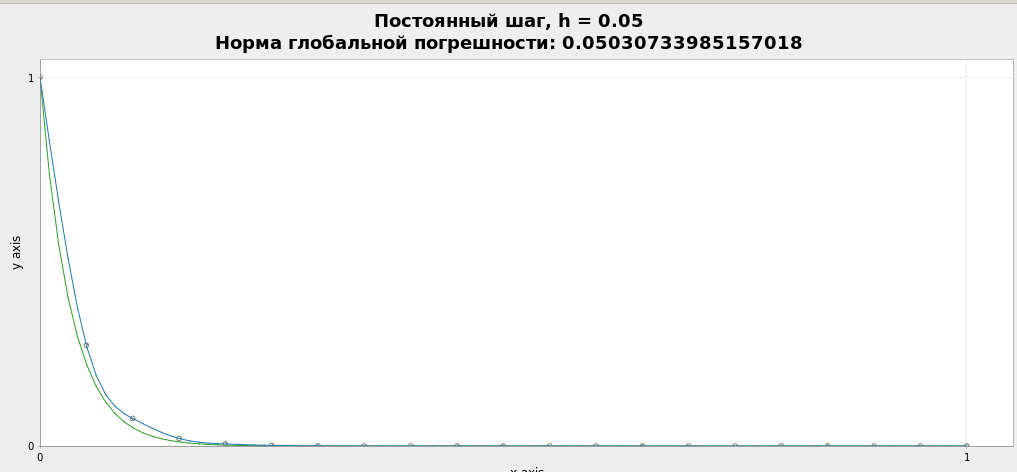
\includegraphics{exp_h_0_05.png}\linebreak\linebreak
      $h = 0.01:$\linebreak\linebreak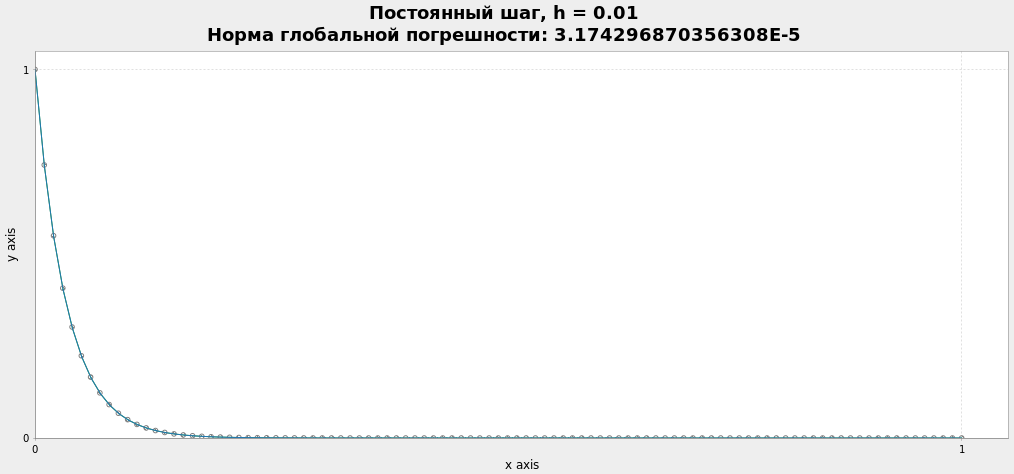
\includegraphics{exp_h_0_01.png}\linebreak\linebreak
      $h = 0.001:$\linebreak\linebreak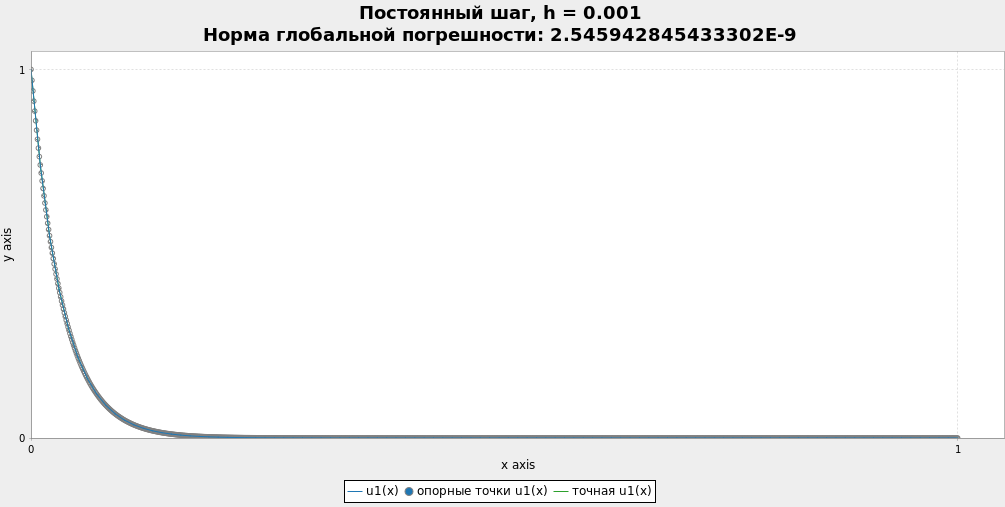
\includegraphics{exp_h_0_001.png}\linebreak\linebreak
      $\epsilon = 0.1:$\linebreak\linebreak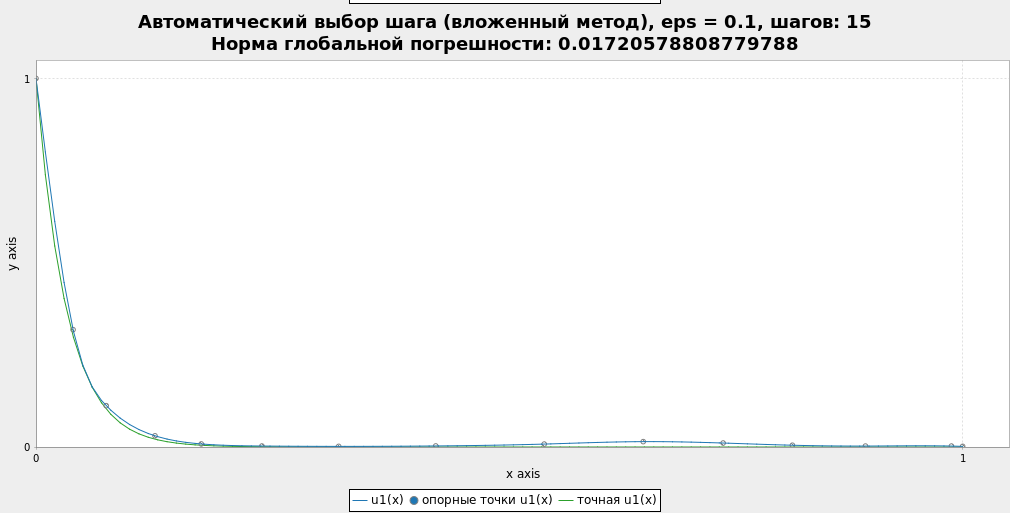
\includegraphics{exp_eps_0_1.png}\linebreak\linebreak
      $\epsilon = 0.01:$\linebreak\linebreak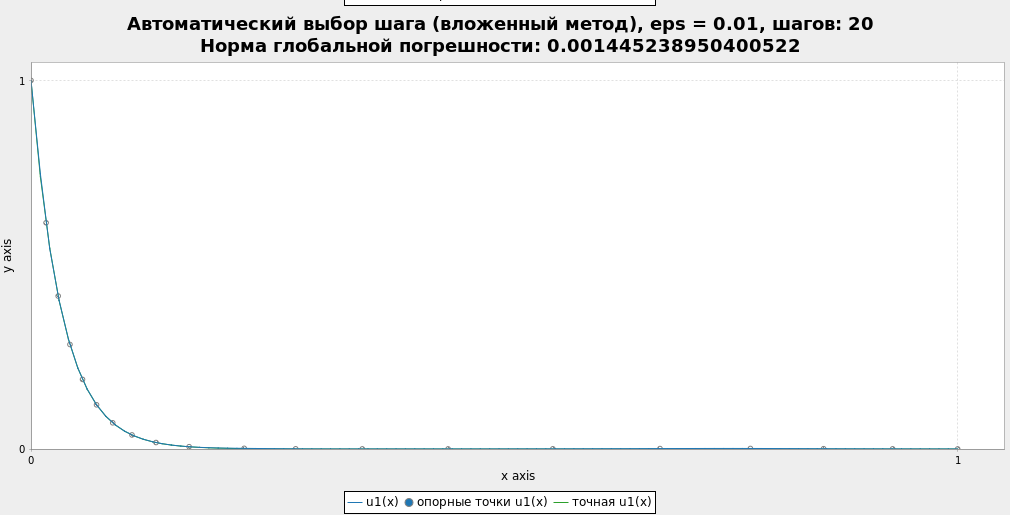
\includegraphics{exp_eps_0_01.png}\linebreak\linebreak
      $\epsilon = 0.001:$\linebreak\linebreak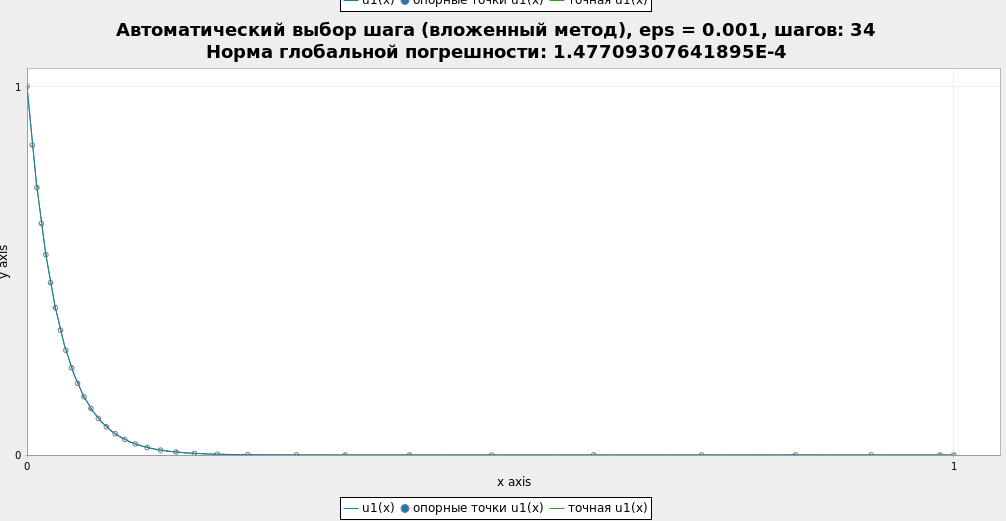
\includegraphics{exp_eps_0_001.png}\linebreak\linebreak
      $\epsilon = 0.0001:$\linebreak\linebreak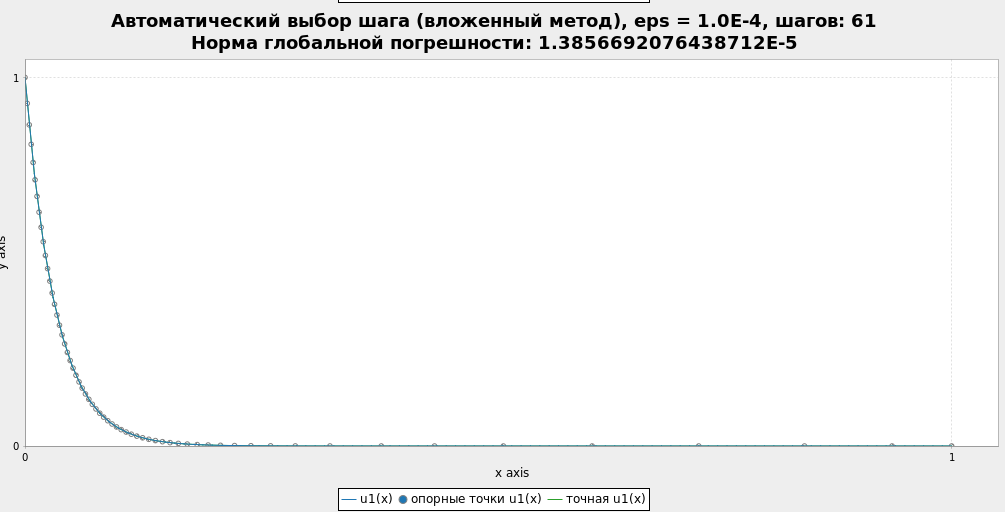
\includegraphics{exp_eps_0_0001.png}\linebreak\linebreak
    \item
      \(u^{'}=\cos{x}+p(u-\sin{x}), 0 \le x \le 6, u(0) = 0\)\linebreak\linebreak
      $p = 1:$\linebreak\linebreak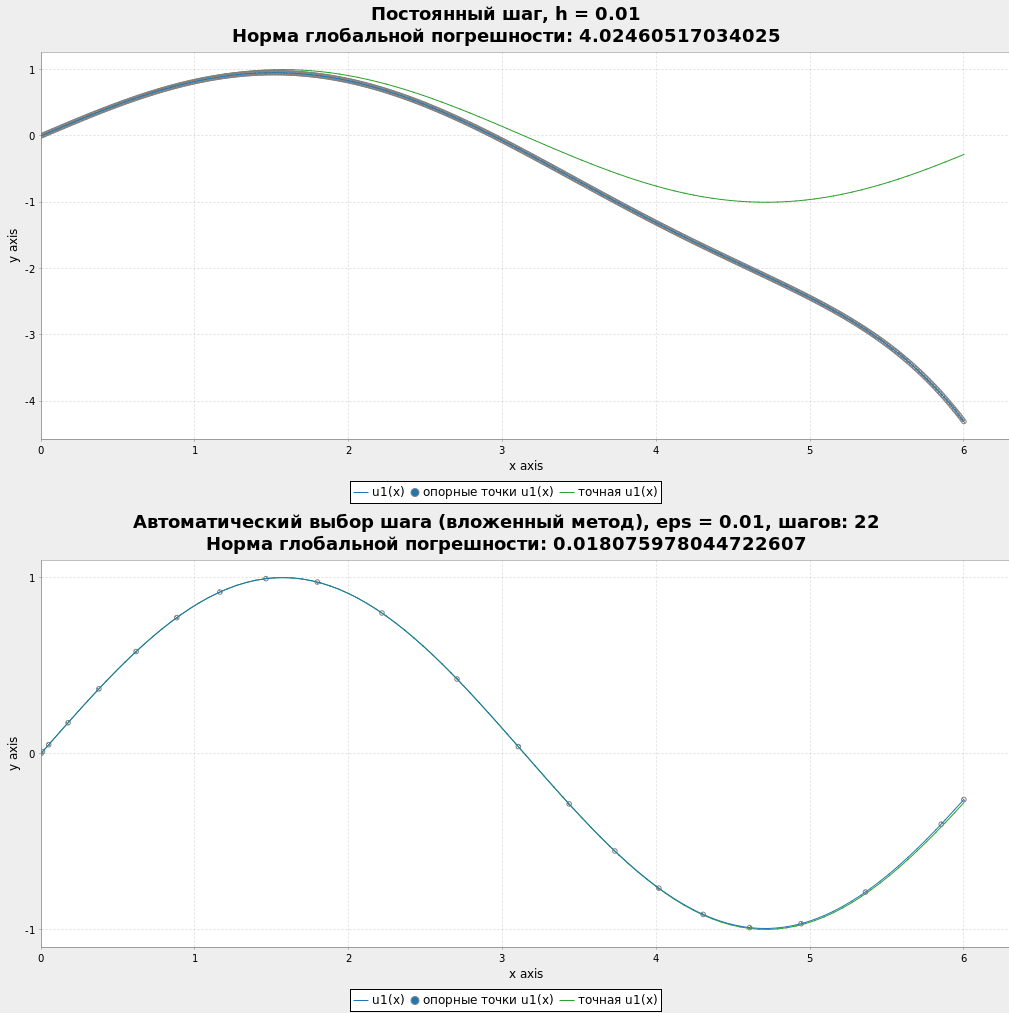
\includegraphics{sc1.png}\linebreak\linebreak
      $p = -1:$\linebreak\linebreak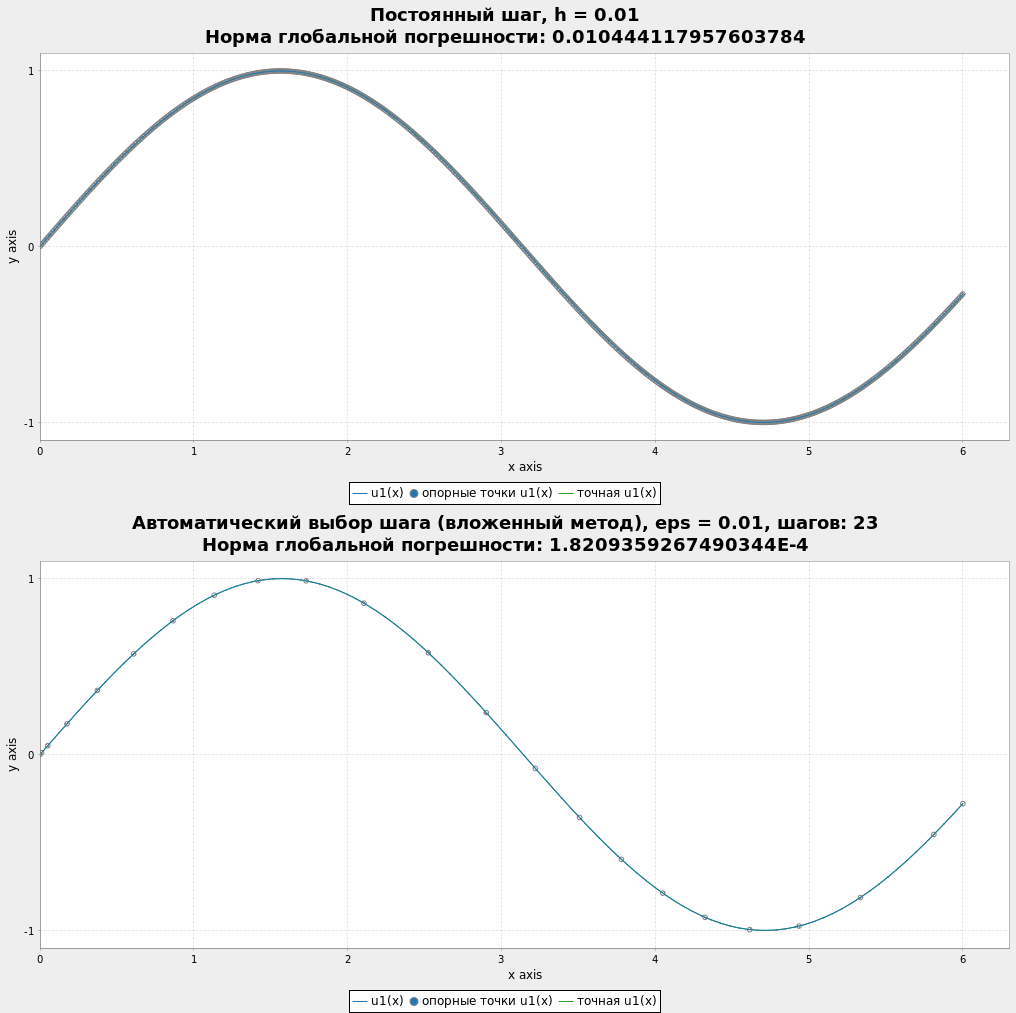
\includegraphics{scm1.png}\linebreak\linebreak
      $p = 0.1:$\linebreak\linebreak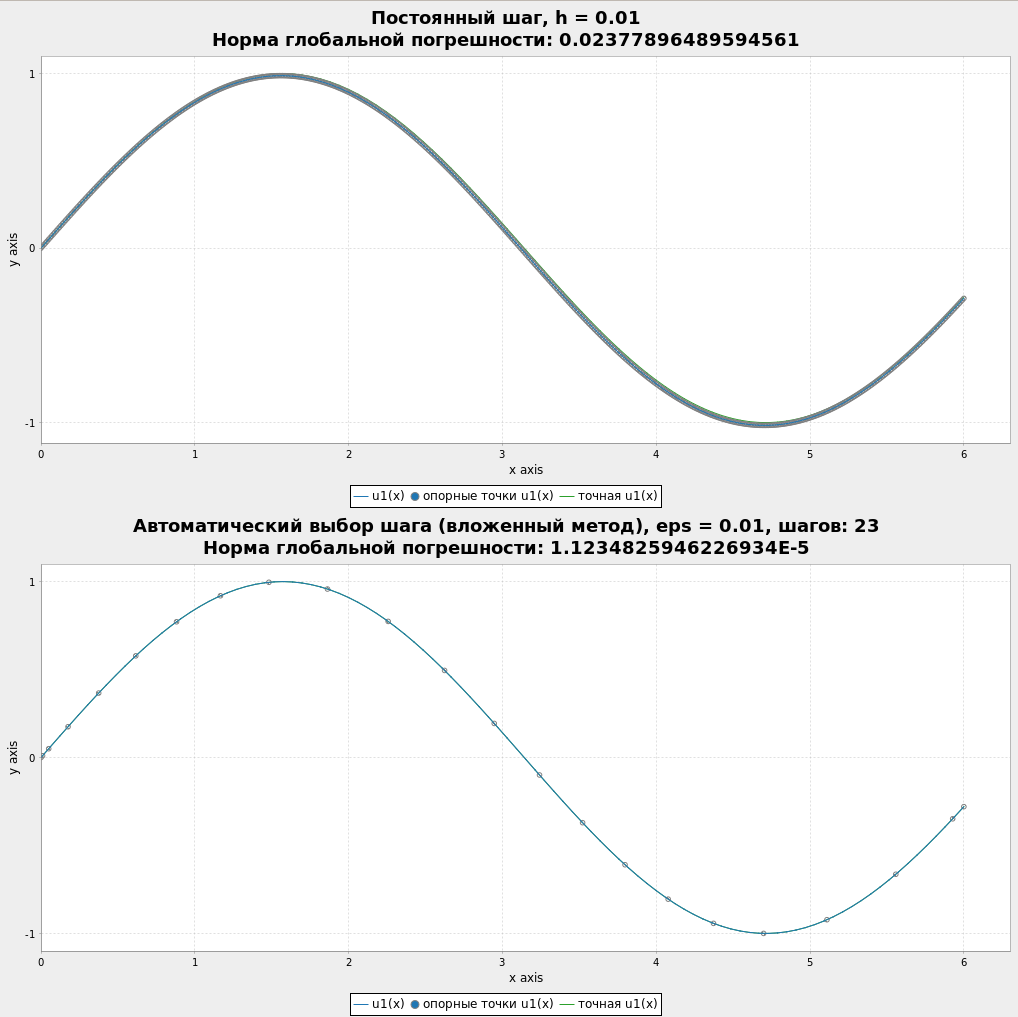
\includegraphics{sc0_1.png}\linebreak\linebreak
      $p = -0.1:$\linebreak\linebreak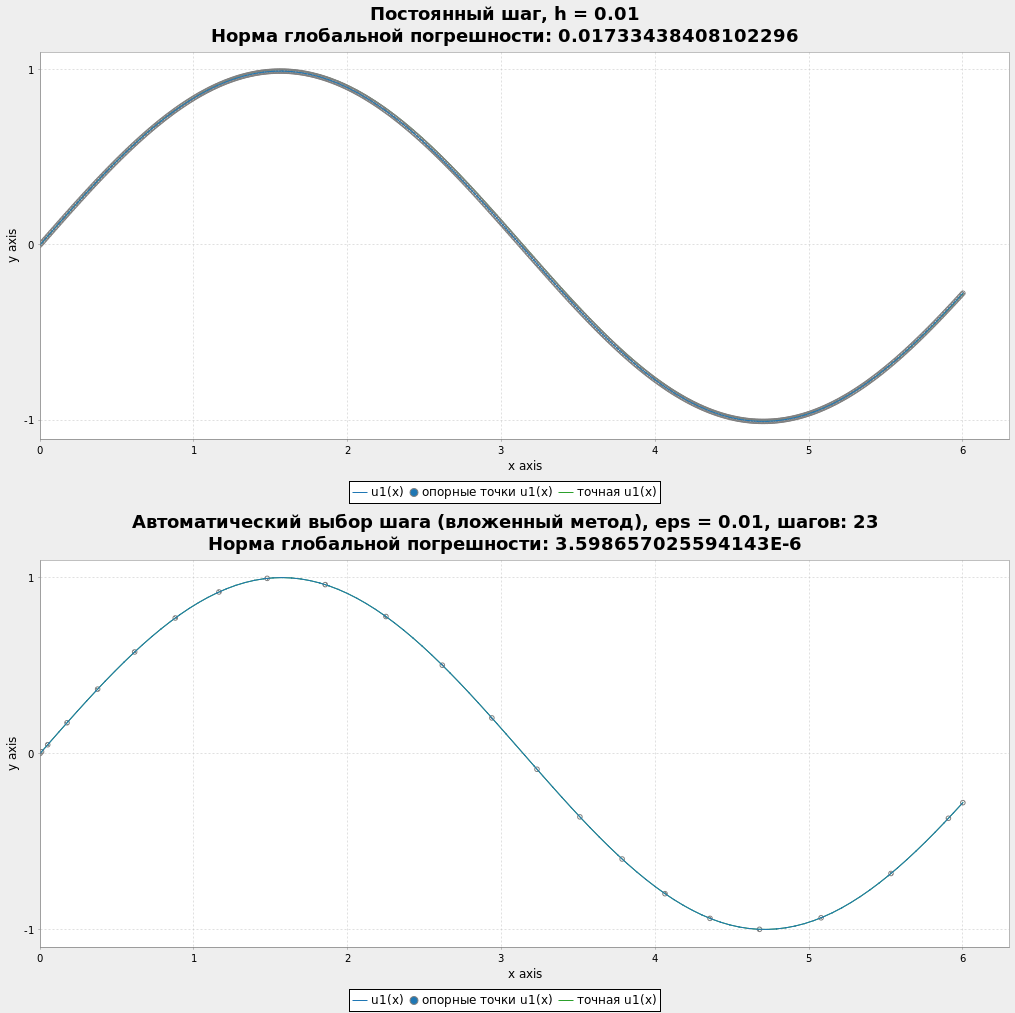
\includegraphics{scm0_1.png}\linebreak\linebreak
      $p = 2:$\linebreak\linebreak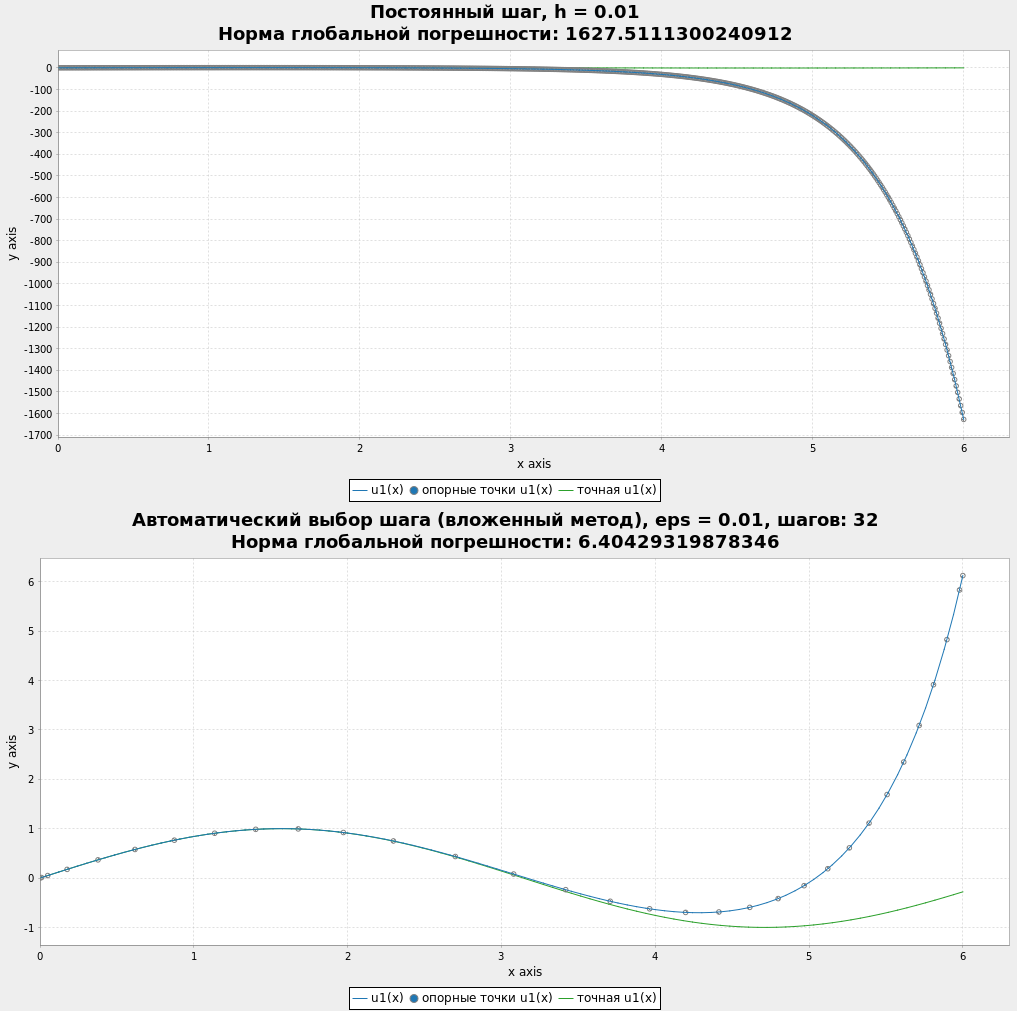
\includegraphics{sc2.png}\linebreak\linebreak
      $p = -2:$\linebreak\linebreak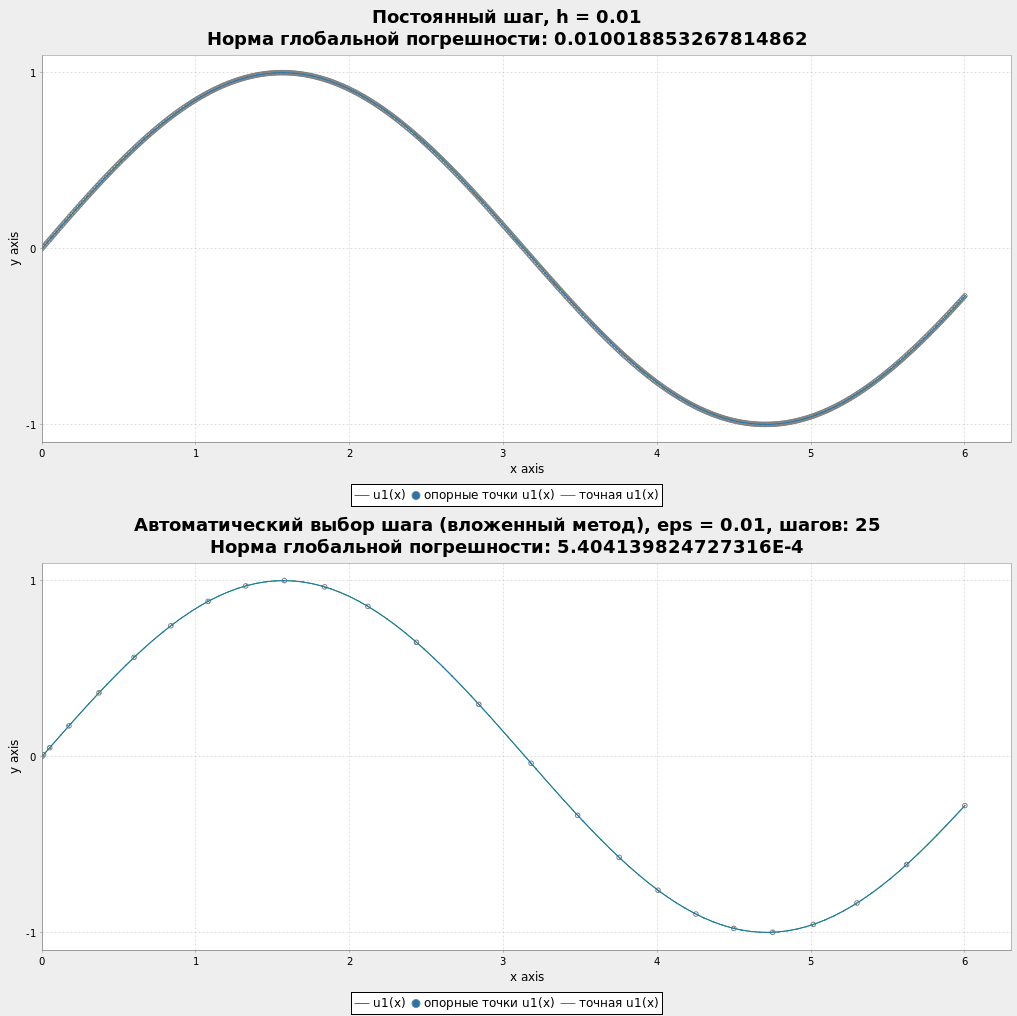
\includegraphics{scm2.png}\linebreak\linebreak
      $p = 5:$\linebreak\linebreak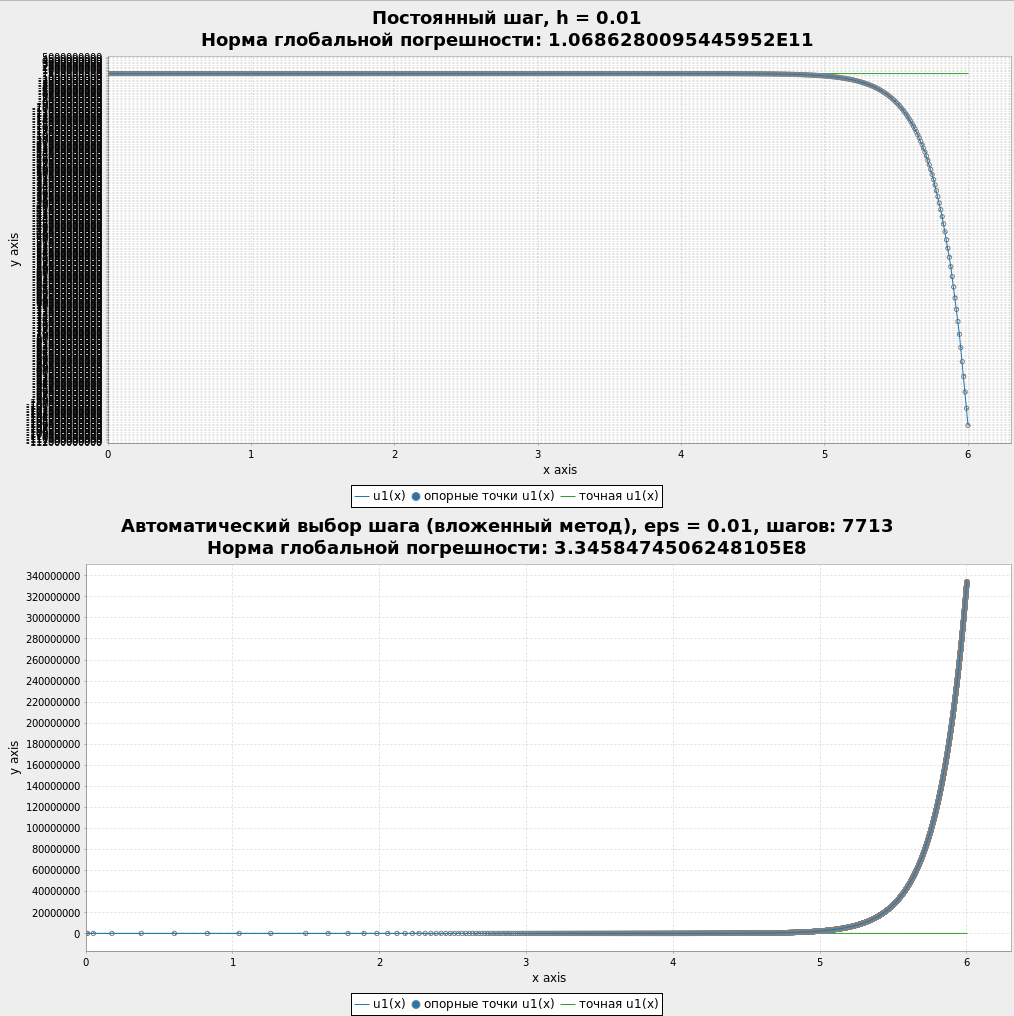
\includegraphics{sc5.png}\linebreak\linebreak
      $p = -5:$\linebreak\linebreak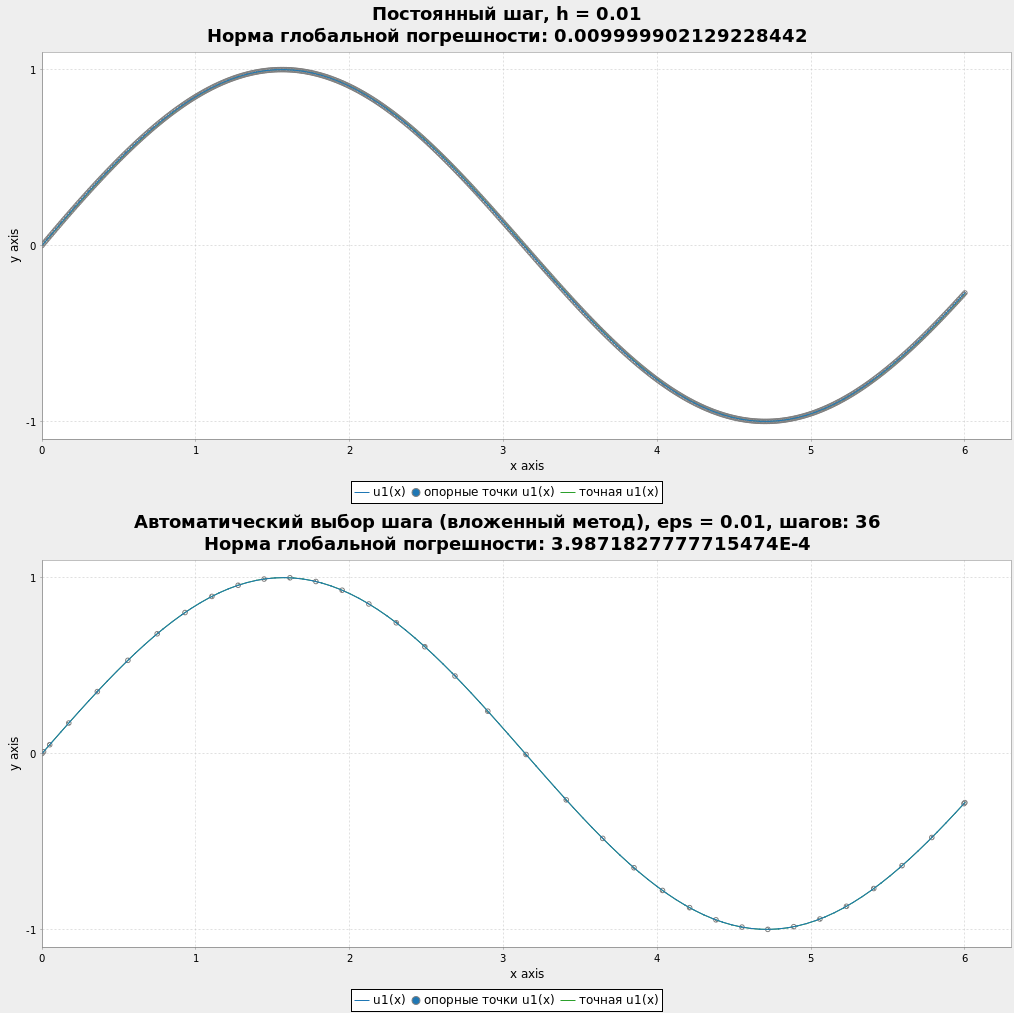
\includegraphics{scm5.png}\linebreak\linebreak
    \item 
      \(u^{'}=2 e^{2x}+p(u-e^{2x}), 0 \le x \le 3, u(0) = 1\)\linebreak\linebreak
      $p = 1:$\linebreak\linebreak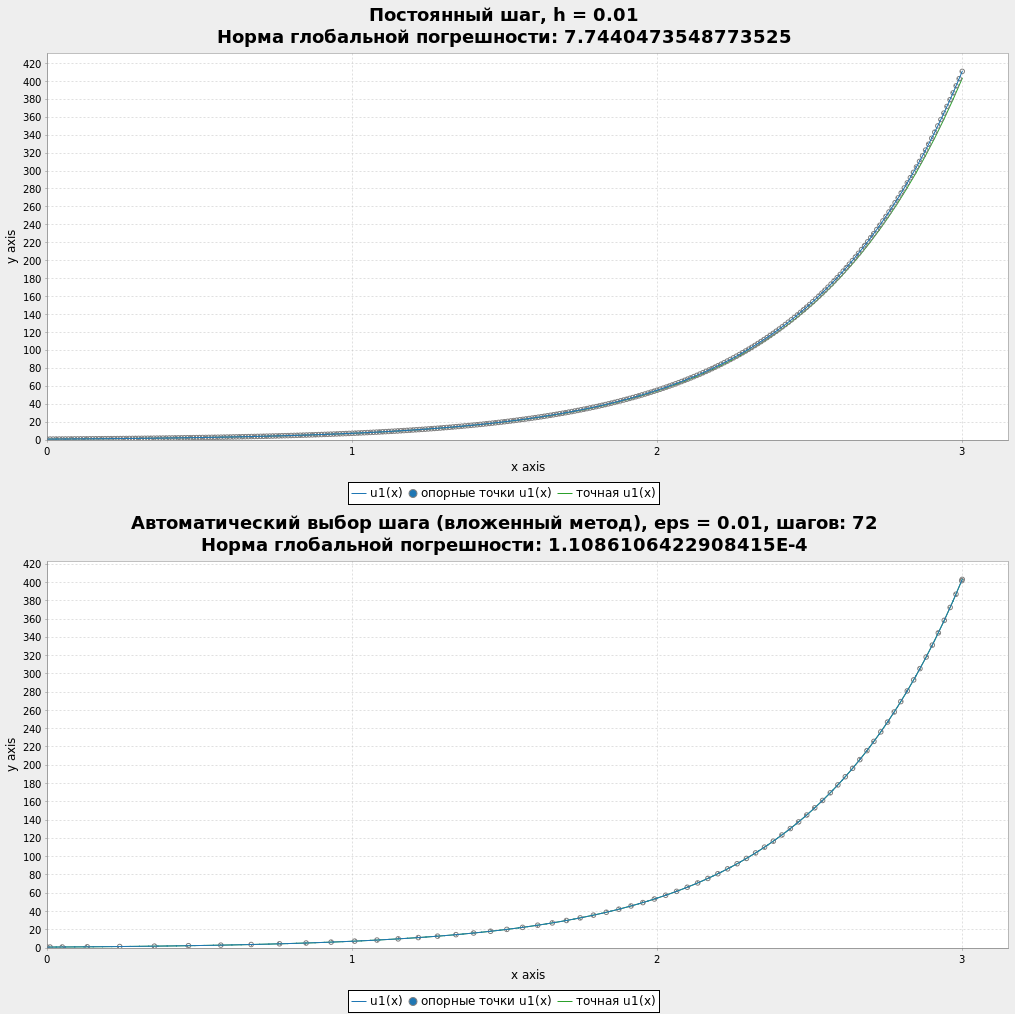
\includegraphics{xp1.png}\linebreak\linebreak
      $p = -1:$\linebreak\linebreak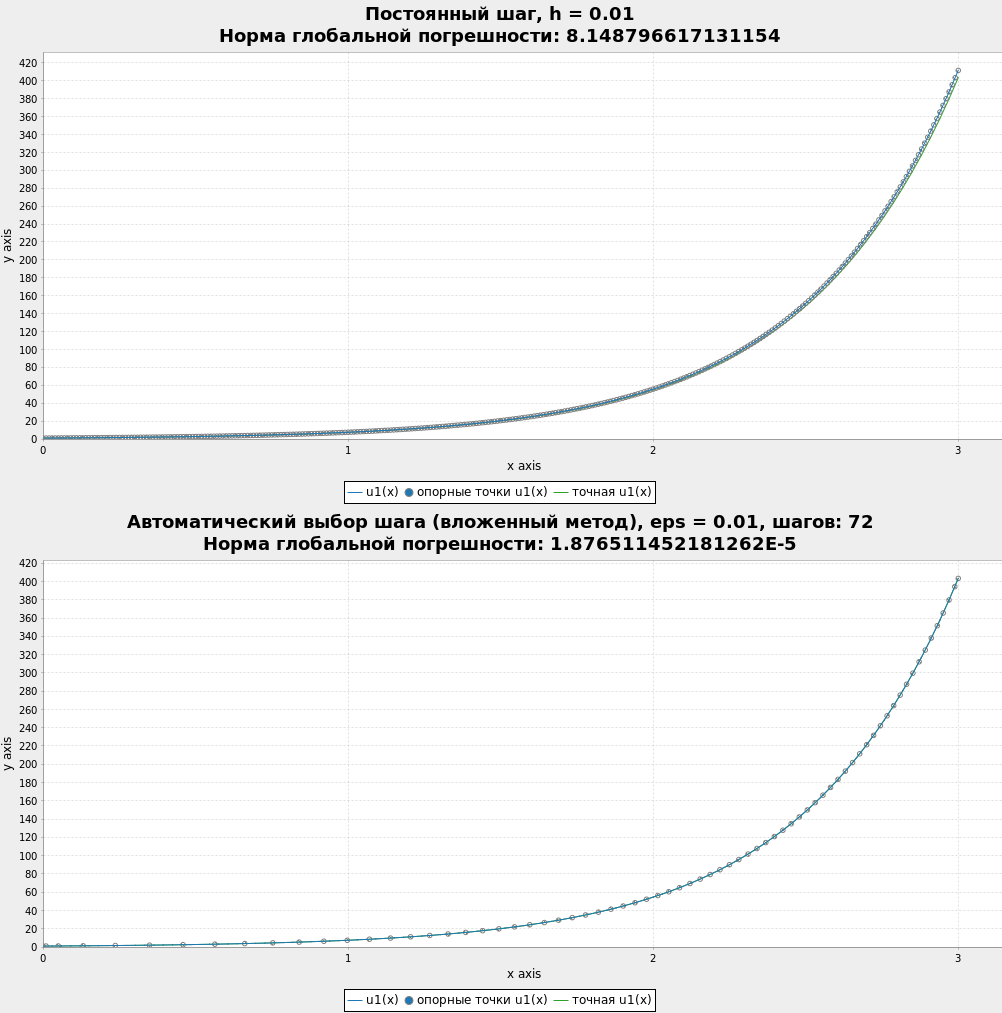
\includegraphics{xpm1.png}\linebreak\linebreak
      $p = 0.01:$\linebreak\linebreak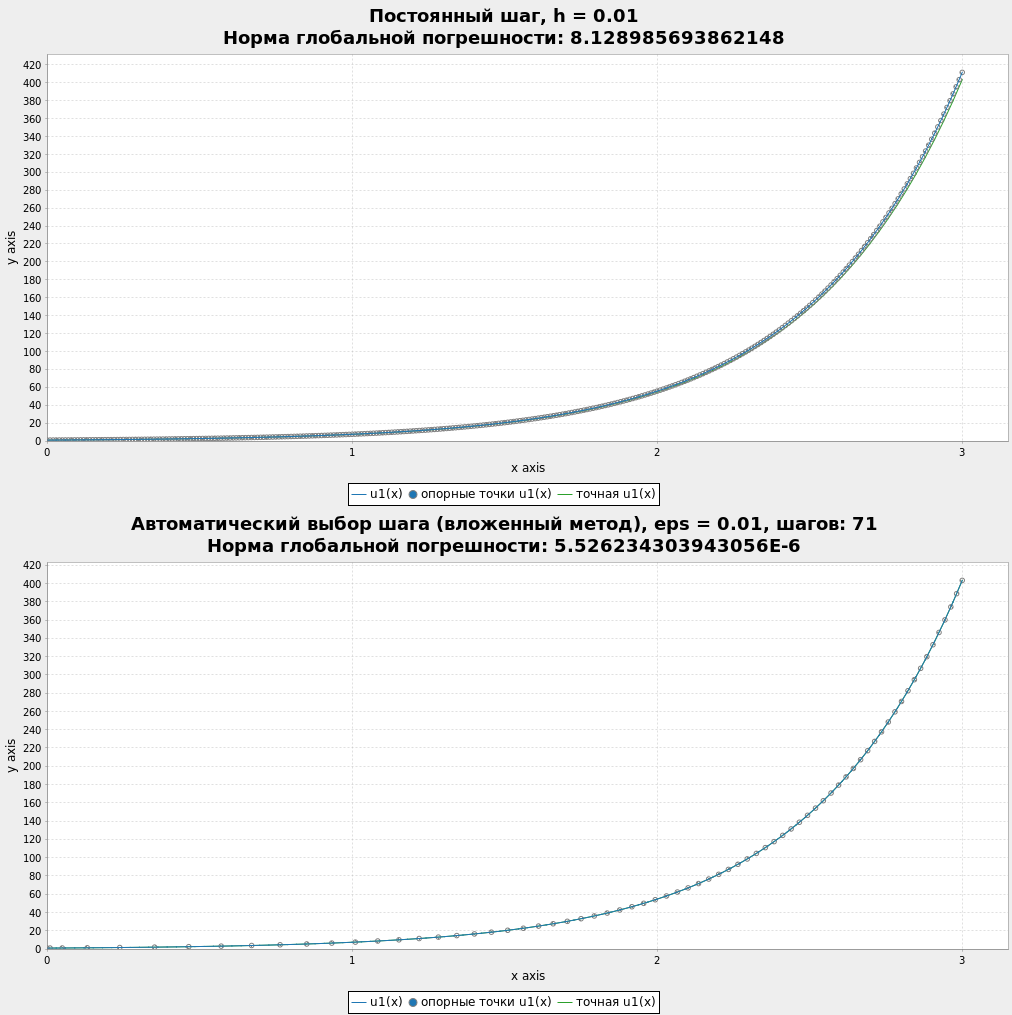
\includegraphics{xp0_01.png}\linebreak\linebreak
      $p = -0.01:$\linebreak\linebreak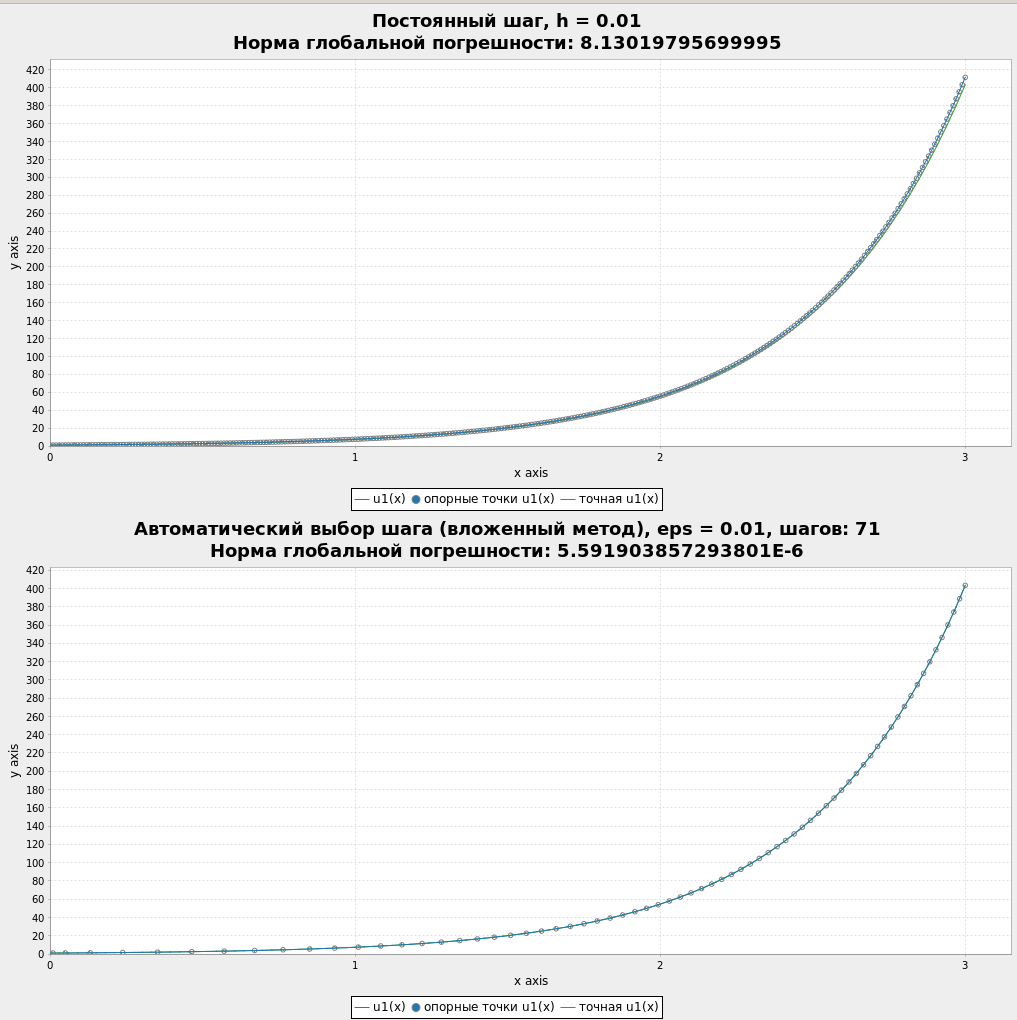
\includegraphics{xpm0_01.png}\linebreak\linebreak
      $p = 2:$\linebreak\linebreak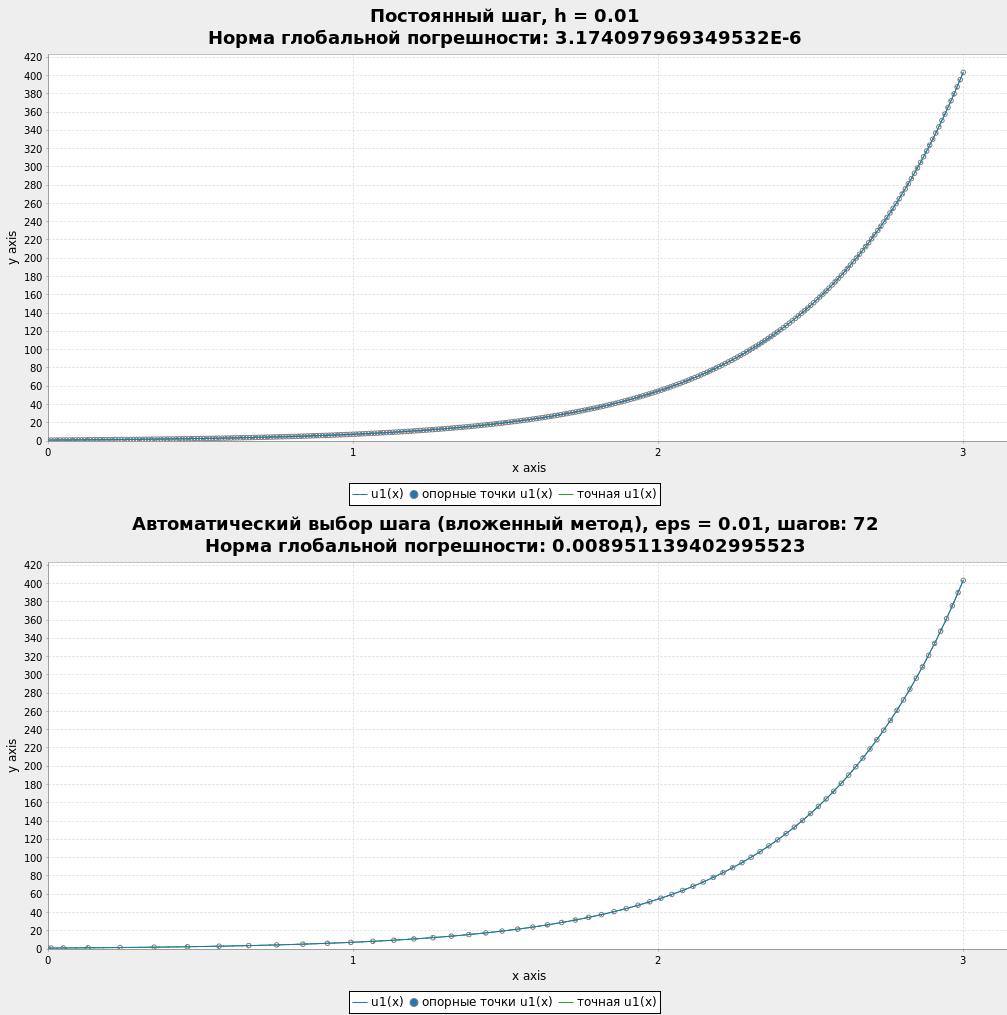
\includegraphics{xp2.png}\linebreak\linebreak
      $p = -2:$\linebreak\linebreak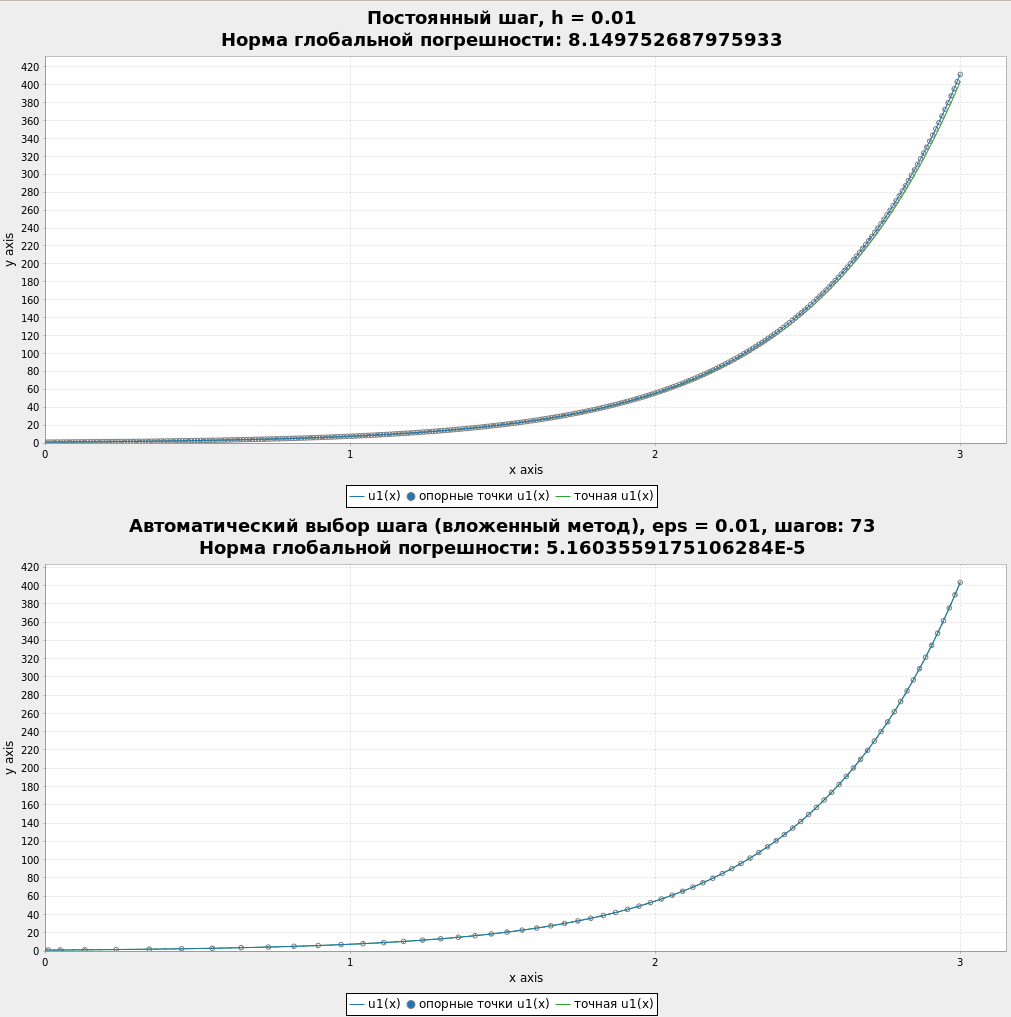
\includegraphics{xpm2.png}\linebreak\linebreak
      $p = 3:$\linebreak\linebreak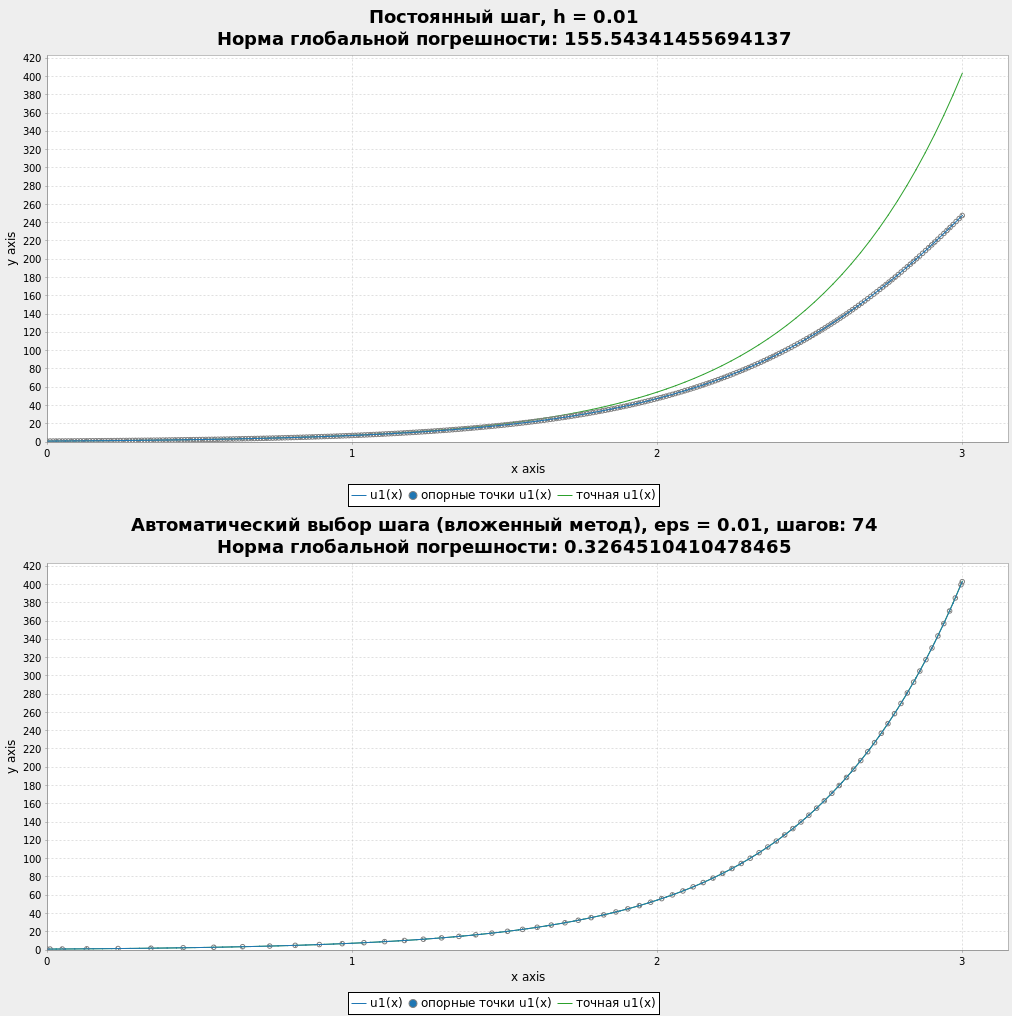
\includegraphics{xp3.png}\linebreak\linebreak
      $p = -3:$\linebreak\linebreak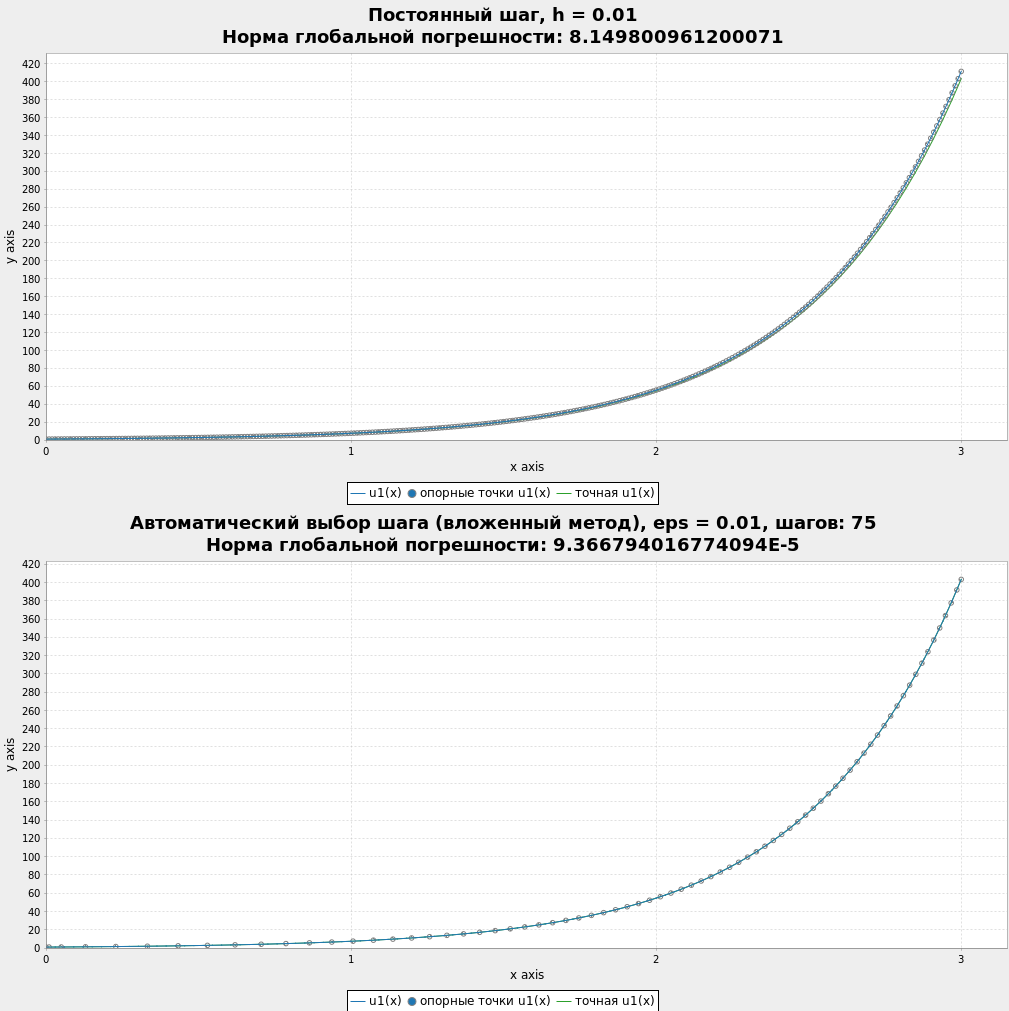
\includegraphics{xpm3.png}\linebreak\linebreak
      $p = 5:$\linebreak\linebreak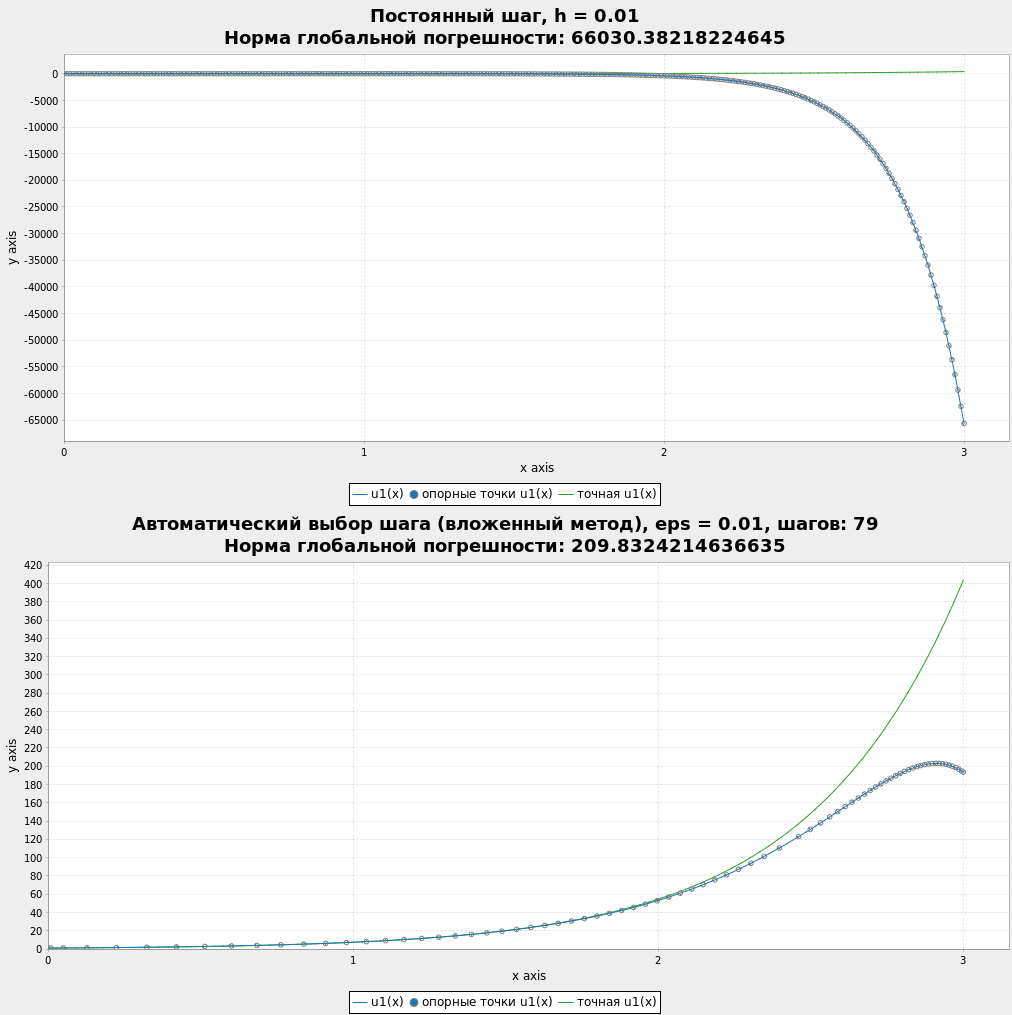
\includegraphics{xp5.png}\linebreak\linebreak
      $p = -5:$\linebreak\linebreak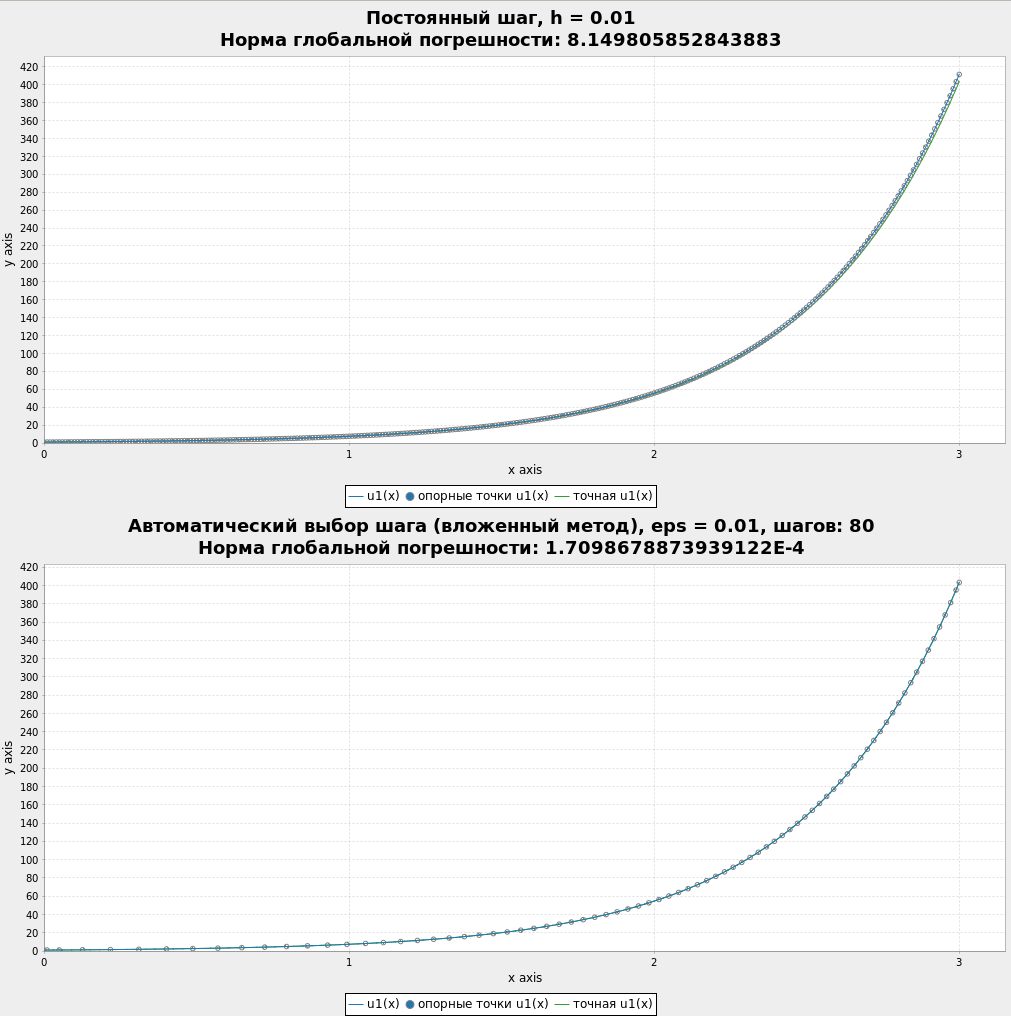
\includegraphics{xpm5.png}\linebreak\linebreak

      Из полученных данных можно сделать вывод, что при $\mathopen|p\mathclose| \rightarrow \infty$ и \(\mathopen|u'\mathclose| > 1\) норма глобальной погрешности неограниченно растёт; чем ближе $u'$ к нулю, тем точнее решение (при прочих равных).

  \end{enumerate}
\end{flushleft}

\end{document}
